% Generated by scripts/make_figures.py.
% Source: experiments/001-attack-spike/FLUENCY_REFERENCE.md.
\begin{figure}[t]\centering
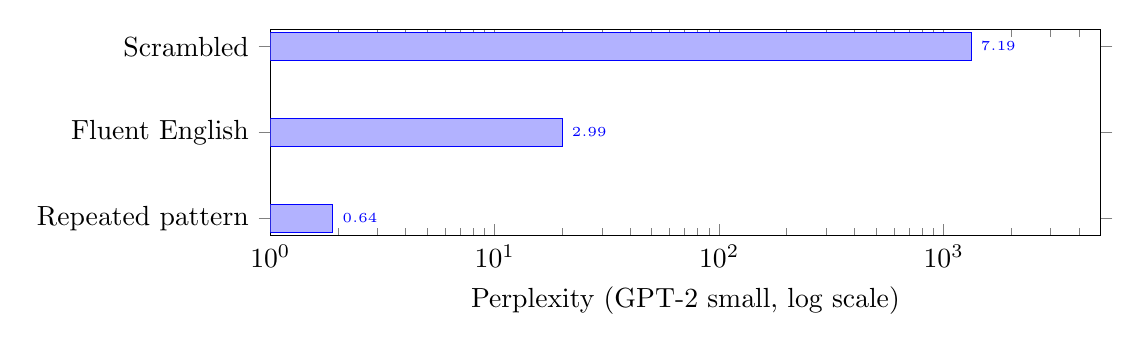
\begin{tikzpicture}
\begin{semilogxaxis}[width=\columnwidth,height=4.2cm,xbar,
  ytick={0,1,2},yticklabels={Repeated pattern,Fluent English,Scrambled},
  xlabel={Perplexity (GPT-2 small, log scale)},xmin=1,xmax=5000,
  nodes near coords,every node near coord/.append style={font=\tiny}]
\addplot coordinates {(1.90,0) (19.98,1) (1326.84,2)};
\end{semilogxaxis}
\end{tikzpicture}
\caption{Measured perplexity of three probe texts under the
independent reference model. The $66\times$ separation between fluent
and scrambled English is the discrimination self-test. The repeated
pattern at 1.90 is the negative result: perplexity rewards repetition,
so the $\rho \le 1.5$ realism bar cannot by itself reject a poison
stream that reuses one passage.}
\label{fig:fluency}
\end{figure}
